\documentclass[../../../../main.tex]{subfiles}
\begin{document}

\begin{flushright}
\footnotesize\textit{【自動文字起こし・要確認】}
\end{flushright}

\noindent
\textbf{[解]} (1) $\angle APB = \alpha, \angle APC = \beta$ とおく。\\
右図のように、$P$ を原点とし、$A$ を $x$ 軸正の方向とする座標をとる。この時、$C$ が $y \ge 0$ にくるようにする。\\
($P$ が $\triangle ABC$ の内部) この時、$\vec{PA}, \vec{PB}, \vec{PC}$ に平行な単位ベクトルを各々 $\vec{a}, \vec{b}, \vec{c}$ として、
\[
\vec{a} = \begin{pmatrix} 1 \\ 0 \end{pmatrix}, \quad \vec{b} = \begin{pmatrix} \cos(-\alpha) \\ \sin(-\alpha) \end{pmatrix}, \quad \vec{c} = \begin{pmatrix} \cos\beta \\ \sin\beta \end{pmatrix}
\]
と書ける。題意から $\vec{a} + \vec{b} + \vec{c} = \vec{0}$ だから、
\[
\begin{cases}
1 + \cos\alpha + \cos\beta = 0 \\
\sin\alpha = \sin\beta
\end{cases}
\quad \cdots \textcircled{1}
\]
$\cos^2\alpha + \sin^2\alpha = 1$ から
\[
2 + 2\cos\beta = 1 \quad \therefore \cos\beta = -\frac{1}{2}
\]
$0 \le \beta \le \pi$ から $\beta = \frac{2}{3}\pi$ で、①から $\alpha = \frac{2}{3}\pi$ が従う。よって、
\[
\angle APB = \frac{2}{3}\pi, \quad \angle APC = \frac{2}{3}\pi \hfill \text{固}
\]

\begin{center}
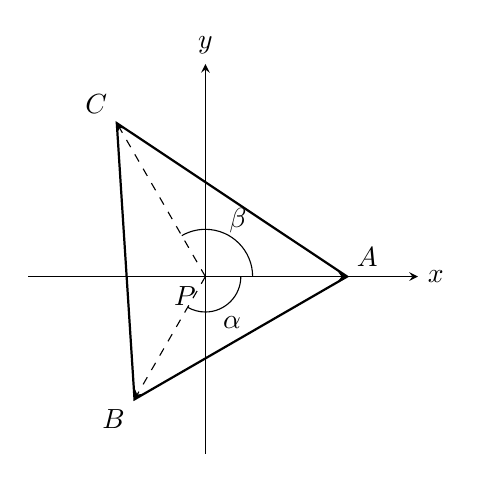
\begin{tikzpicture}[scale=1.5, >=stealth]
  \draw[->] (-1.5,0) -- (1.8,0) node[right] {$x$};
  \draw[->] (0,-1.5) -- (0,1.8) node[above] {$y$};
  \node[below left] at (0,0) {$P$};
  
  \coordinate (A) at (1.2, 0);
  \coordinate (B) at ({-1.2*cos(60)}, {-1.2*sin(60)});
  \coordinate (C) at ({-1.5*cos(60)}, {1.5*sin(60)});
  
  \draw[thick] (A) -- (B) -- (C) -- cycle;
  \draw[dashed, ->] (0,0) -- (A) node[above right] {$A$};
  \draw[dashed, ->] (0,0) -- (B) node[below left] {$B$};
  \draw[dashed, ->] (0,0) -- (C) node[above left] {$C$};
  
  \draw (0.4,0) arc (0:120:0.4);
  \node at (60:0.55) {$\beta$};
  \draw (0.3,0) arc (0:-120:0.3);
  \node at (-60:0.45) {$\alpha$};
\end{tikzpicture}
\end{center}

\noindent
(2) $|\vec{PA}| = a, |\vec{PB}| = b, |\vec{PC}| = c$ とすると、
\[
\vec{PA} = a \begin{pmatrix} 1 \\ 0 \end{pmatrix}, \quad \vec{PB} = -\frac{b}{2} \begin{pmatrix} 1 \\ \sqrt{3} \end{pmatrix}, \quad \vec{PC} = \frac{c}{2} \begin{pmatrix} -1 \\ \sqrt{3} \end{pmatrix}
\]
である。したがって、
\[
\vec{AB} = \begin{pmatrix} -\frac{1}{2}b - a \\ -\frac{\sqrt{3}}{2}b \end{pmatrix}, \quad \vec{AC} = \begin{pmatrix} -\frac{1}{2}c - a \\ \frac{\sqrt{3}}{2}c \end{pmatrix}
\]
だから、$\angle CAB = \frac{\pi}{2}, AB = 1, AC = \sqrt{3}$ から、
\[
\begin{cases}
(-\frac{1}{2}b - a)(-\frac{1}{2}c - a) - \frac{3}{4}bc = 0 \\
(\frac{1}{2}b + a)^2 + \frac{3}{4}b^2 = 1 \\
(\frac{1}{2}c + a)^2 + \frac{3}{4}c^2 = 3
\end{cases}
\iff
\begin{cases}
a^2 + b^2 + ab = 1 \\
a^2 + c^2 + ac = 3 \\
a^2 + \frac{1}{2}(ac + ab - bc) = 0
\end{cases}
\]
これをといて、
\[
a = \frac{\sqrt{7}}{7}, \quad b = \frac{2\sqrt{7}}{7}, \quad c = \frac{4\sqrt{7}}{7} \hfill \text{固}
\]

\bigskip

\end{document}
